Delu aplikacije koji je vezan za dobijanje licenci mogu da pristupe administrator, klijent i recepcioner. Svako od njih može da vidi opise postojećih programa obuke. A dodatno, u zavisnosti od toga koji korisnik sistema je ulogovan, ova sekcija nudi različite opcije.

Administrator može da vidi dugme "Dodaj novi program obuke" pomoću koga se otvara formular za unos informacija o novom programu obuke. Nakon popunjavanja formulara može odabrati opciju "Dodaj" čime se proverava da li su uneti svi potrebni podaci. Ukoliko nisu, administrator se obaveštava o tome i daje mu se mogućnost da popuni preostala polja. Ukoliko u bilo kom trenutku, administrator želi da odustane od dodavanja novog programa, može kliknuti dugme "Odustani" čime se brišu sve prethodno unete informacije i zatvara se formular. Izgled ovog segmenta, može se videti na slikama \ref{fig:novi_program1} i \ref{fig:novi_program2}.
Administrator ima i opciju unosa rezultata ispita. Klikom na dugme "Objavi rezultate ispita" ispod opisa nekog programa obuke, prelazi se na stranicu koja sadrži formular za unos ocena. Na stranici će već biti prikazan spisak klijenata koji su prijavljeni na taj program, a administrator samo treba u odgovarajuća polja da unese njihove ocene i informaciju o tome da li dobijaju licencu. Izgled formulara je prikazan na slici \ref{fig:admin_ispiti}.

\begin{figure}[!ht]
\begin{center}
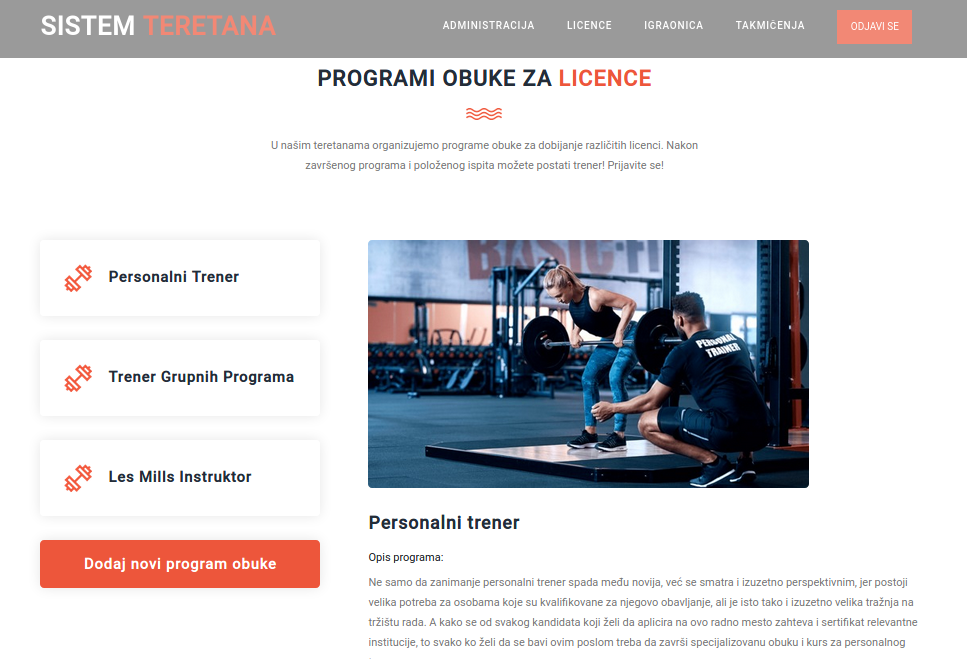
\includegraphics[scale=0.30]{sections/korisnicki_interfejs/screenshots/licenca-admin.png}
\end{center}
\caption{Dodavanje novog programa obuke}
\label{fig:novi_program1}
\end{figure}

\begin{figure}[!ht]
\begin{center}
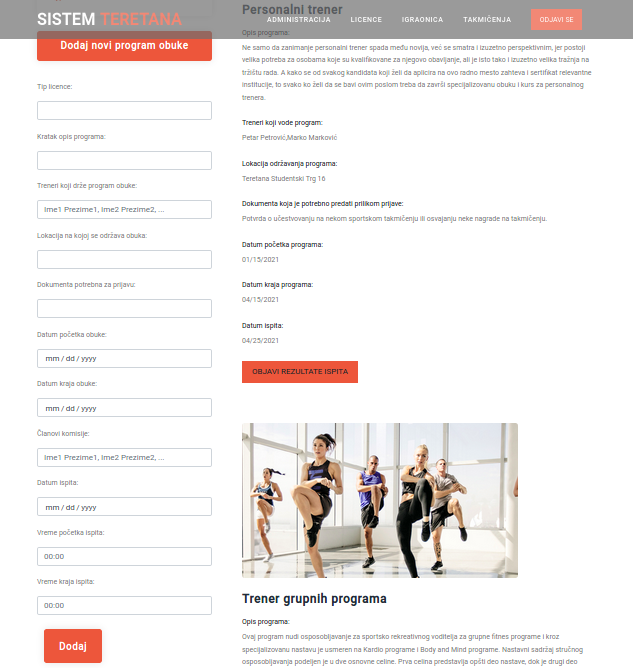
\includegraphics[scale=0.60]{sections/korisnicki_interfejs/screenshots/licenca-admin-nov-program.png}
\end{center}
\caption{Dodavanje novog programa obuke - forma}
\label{fig:novi_program2}
\end{figure}

\begin{figure}[!ht]
\begin{center}
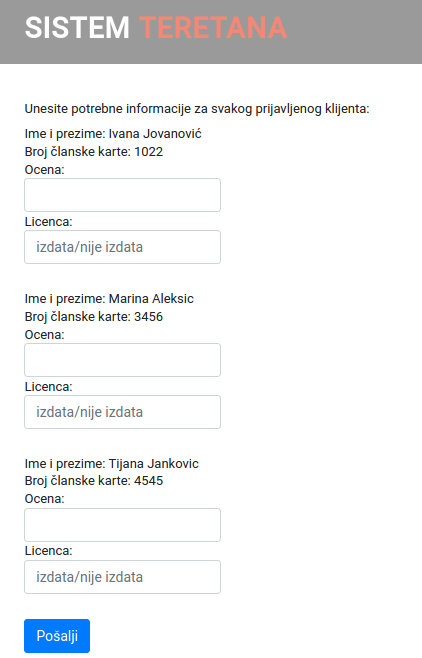
\includegraphics[scale=0.45]{sections/korisnicki_interfejs/screenshots/licenca-admin-ispiti.png}
\end{center}
\caption{Formular za unos rezultata ispita}
\label{fig:admin_ispiti}
\end{figure}

Klijent može da se prijavi na program obuke klikom na dugme "Prijavi se", ispod koga će se otvoriti formular koji je potrebno popuniti. Klijent u svakom trenutku može da odustane od popunjavanja prijave klikom na dugme "Odustani". Klijent takođe može da pogleda rezultate ispita svakog od programa klikom na dugme "Rezultati ispita", čime se prelazi na stranicu koja sadrži sve potrebne informacije za rezultate datog programa. Formular za prijavu se nalazi na slici \ref{fig:licenca_klijent_prijava}, a stranica za prikaz rezultata na slici \ref{fig:licenca_klijent_ispiti}.

\begin{figure}[!ht]
\begin{center}
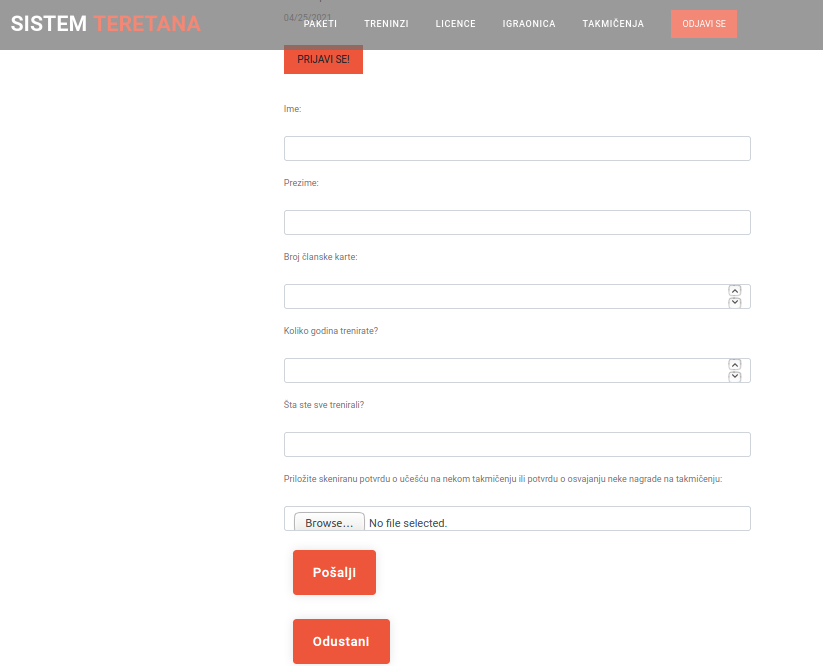
\includegraphics[scale=0.45]{sections/korisnicki_interfejs/screenshots/licenca-klijent-prijava.png}
\end{center}
\caption{Formular za prijava klijenta na program obuke}
\label{fig:licenca_klijent_prijava}
\end{figure}

\begin{figure}[!ht]
\begin{center}
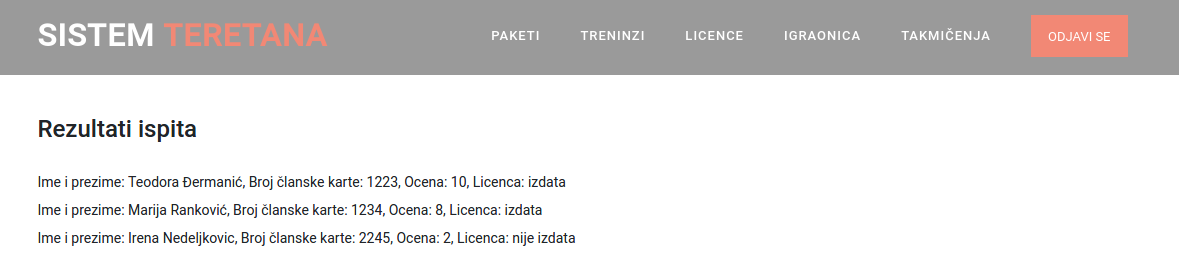
\includegraphics[scale=0.25]{sections/korisnicki_interfejs/screenshots/licenca-klijent-ispiti.png}
\end{center}
\caption{Rezultati ispita}
\label{fig:licenca_klijent_ispiti}
\end{figure}


Recepcioner ima mogućnost prijave klijenta na program obuke. Klikom na dugme "Prijavi klijenta" otvara se odgovarajući formular, koji izgleda slično kao i formular za samostalnu prijavu klijenta.